\section{Evaluation}
\label{sec:evaluation}

We evaluate \tool by comparing the performance of three programs: A word count with prior text parsing, TPCH query 12 and a k-means application that uses an array processing extension for \tool. \\

All experiments were performed on the Amazon EC2 Cloud, using 20 "m1.large" nodes as slaves and one as master. They each have 7.5 Gb of memory, 2 virtual cores with 2 EC2 compute units each, 850 Gb of instance storage and provide high network throughput. Prior to the experiments we have measured up to 50 MB/s between two nodes. For the Hadoop experiments we used current Cloudera Hadoop distribution cdh3u4. We used Crunch version 0.2.4 and Scoobi 0.4.0. We did not tweak Hadoop configuration beyond the default settings. For benchmarking Spark we used the Mesos \cite{hindman_mesos:_2011} EC2 script to start a cluster, and the most recent version of Spark for our tests. For Spark we changed the default parallelism level to the number of cores in the cluster and increased the available memory to 6GB. 

% Regular expressions
For a fairer comparison with Pig we adapted some of their regular expression optimizations for our program. Pig makes use of a faster library \cite{mollerdk} and implements an optimized splitting function when the regular expression becomes a simple comparison of one character. We implemented a frontend for regular expressions which automatically selects the best variant for each expression and operation. 

We were also getting unsatisfying numbers from our Scoobi backend, so we added Crunch in about one week. This really shows that it is easy to add a new backend, and the modularity allows us to reuse pieces of other backends. Crunch's implementation of join performed very badly in local benchmarks, so we replaced it with our own one for these benchmarks.

% Data Serialization
For serialization of data we used LMS code generation to achieve minimal overhead for both Crunch and Scoobi frameworks. We used generated versions since they outperformed the Kryo framework by a thin margin. For Spark we used Kryo. All benchmarks were run three times and in the figures we present only the average. We also computed the standard deviations but we omitted them since they are smaller than 3\% in all experiments.

\begin{figure}[!hbt]
    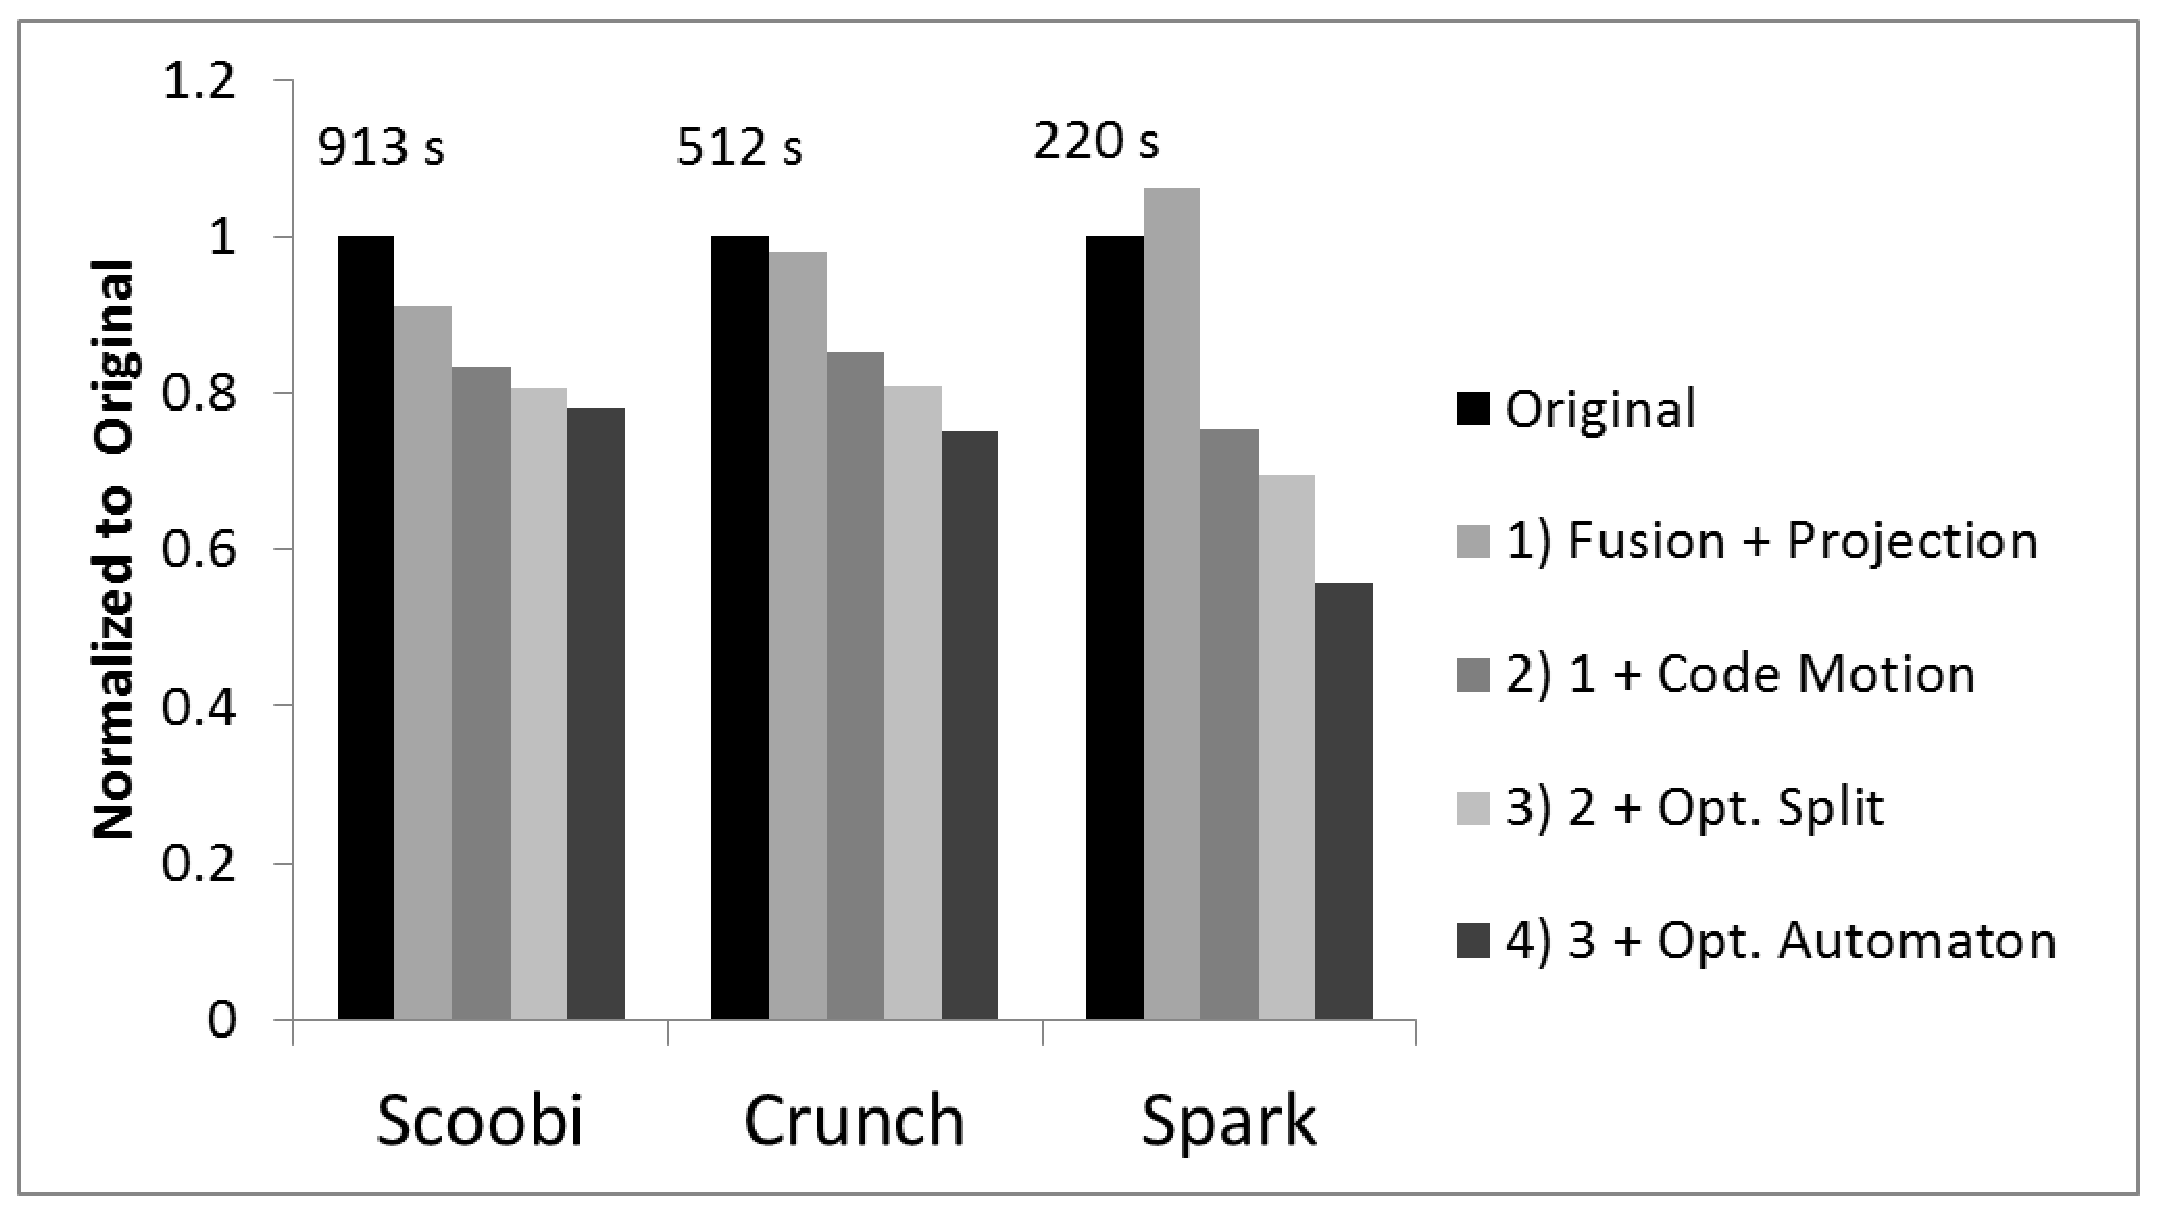
\includegraphics[width=8.6cm]{figures/word-count}
   \caption{Word Count benchmark.}
   \label{fig:word-count}%\vspace{10pt}
\end{figure}

\begin{figure}[!hbt]
    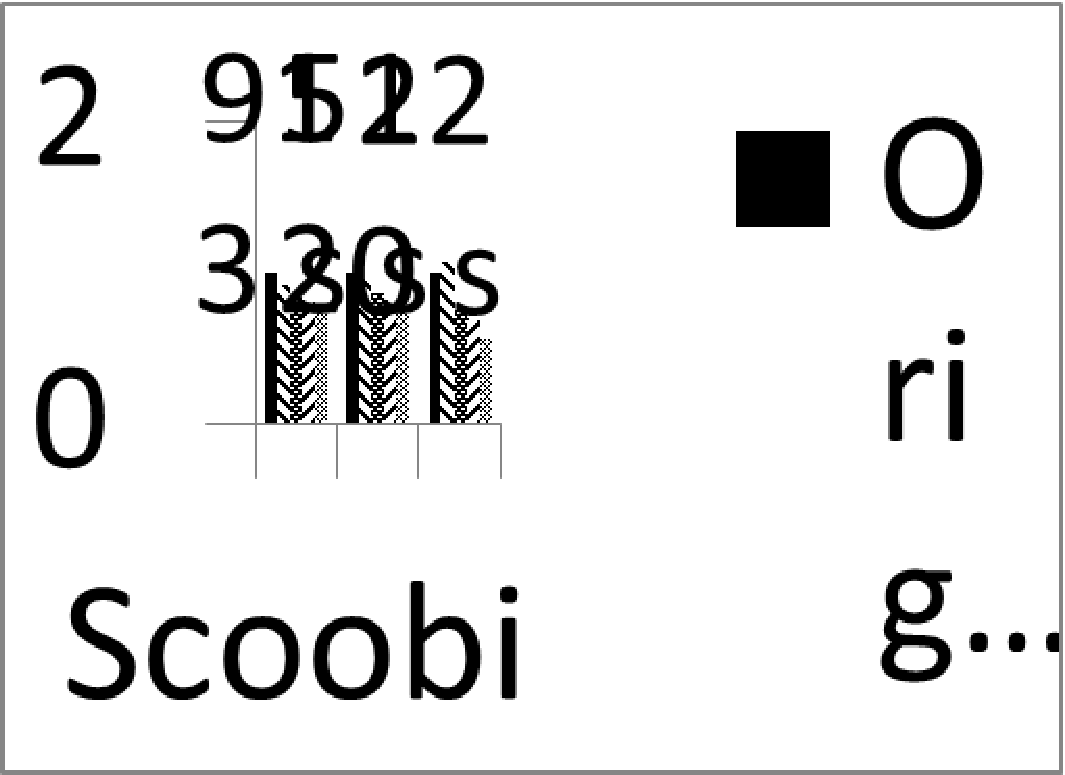
\includegraphics[width=8.6cm]{figures/k-means}
   \caption{K-means benchmark.}
   \label{fig:k-means}%\vspace{10pt}
\end{figure}

\begin{figure}[!hbt]
    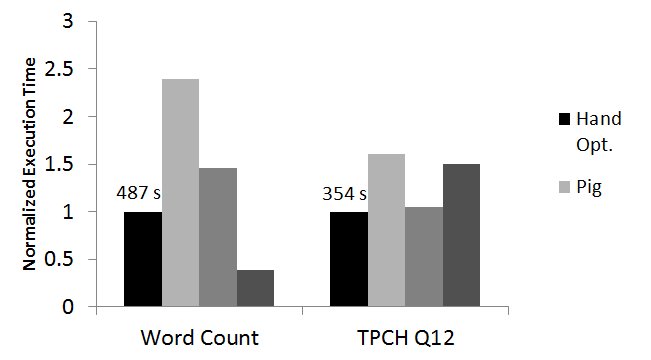
\includegraphics[width=8.6cm]{figures/pig}
   \caption{Comparison with Pig.}
   \label{fig:pig}%\vspace{10pt}
\end{figure}

\begin{figure}[!hbt]
    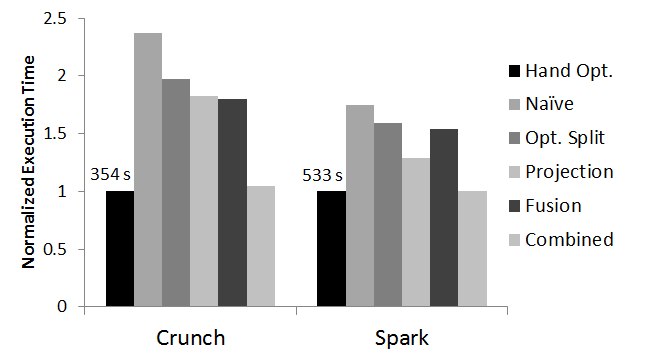
\includegraphics[width=8.6cm]{figures/tpch}

   \caption{TPCH query 12 benchmark.}
  \label{fig:tpch}%\vspace{10pt}    
\end{figure}

% WordCount
\subsection{Parsing and Word Count}
\label{subsec:parsing-word-count}
\todo{Stivo explain the regular expressions and what do we want to prove}
Our input is a 62 GB set of freebase wikipedia data. Our benchmark tries to clean up the input which is not properly parsed. It uses 5 regular expressions in total to split, replace and match on strings. It can not benefit from field reduction and it only requires one shuffle stage with little data involved, so its performance is a good indication of the cpu time spent on the mapper part of the computation.

For this evaluation we start with an unoptimized version and add optimizations one by one. We first add our loop fusion and field reduction optimizations. We then switch our DSL to use reusable patterns, which allows code motion to move them out of the loop and only compile them once. Next we add the fast splitter and for the fully optimized version we use the faster regex library. 

In figure \ref{fig:word-count} we show the job times for these versions normalized to the unoptimized program version. Performance improvements are from \todo{75-82} in Scoobi, \todo{Crunch} and in Spark. The base performances of the frameworks differ by a large margin for this benchmark. Scoobi profits the most in this case from the fusion and projection optimization which indicates that the framework imposes additional overhead for declarative operations.

In Spark, we notice a larger benefits from our optimizations. We believe that it has significantly smaller IO overhead so that the optimizations have a bigger effect. Also, we notice that fusion optimization and field reduction is slower than the original program, but only in Spark. This result does not match our experiments in a smaller cluster setup, we believe that it could be caused by a straggler node in the cloud environment.

% TPCH q12
\subsection{TPCH Query 12}
\label{subsec:tpch-query-12}

To evaluate effects of projection insertion we have run the TPCH \cite{tpch} query 12  which includes an expensive \code{join} operation and aggregates the whole result to just two values. As the data set we use a 100 GB input data set generated by the DbGen generator \cite{tpch}.

In figure \ref{fig:tpch} we show job times for different optimizations normalized to the unoptimized program version on different frameworks. We notice that projection insertion gives 20\% percent better performance on Crunch and 11\% on Scoobi. On Spark, the projection insertion improves the performance by 40\%, significantly more than for the Hadoop based frameworks. We believe the difference to be because Hadoop spills the data to disk earlier, while Spark tries to keep it in the memory until it has to spill it. Spark is therefore very sensitive to memory pressure, but the authors have already announced a more efficient spill handling.
%We believe that either network shuffle or the \code{join} operation are less optimal in Spark. 
In this benchmark we can also see how the optimizations we implemented interact with each other. The absolute performance gain for combined optimizations is 3\% greater for Crunch, equal for Scoobi and 9\% smaller for Spark than the sum of the absolute individual gains.

\subsection{Comparison with Pig}
\label{subsec:pig}
% Pig Comparison

In figure \ref{fig:pig} we compare most optimal versions of benchmarks to equivalent Pig programs. The figure is normalized to the Pig execution time and overall job time is stated above the bar. We notice that for TPCH query 12 the combination of fusion, code motion and field reduction outperform Pig when the Crunch framework is used. 
%I don't like this analysis.
For Crunch, field reduction alone is not enough to outperform the Pig framework. We believe that this result is caused by more efficient join operation in Pig. In future work we will investigate the cause for this.
In the Word Count Crunch outperforms Pig even without any optimizations applied. With all optimizations the difference is significant. We explain this by the more optimal regular expressions processing support included in \tool. In regular expressions used in the benchmark Pig falls back to default Java regular expressions while \tool uses optimized automaton library. Scoobi framework performs slower than Pig in both benchmarks even with all optimizations applied.

\todo{go up}
For the sake of showing comparison between the Hadoop based frameworks and the Spark framework we include the Spark results in the graph. We see that in all cases except for unoptimized TPCH query 12 it significantly outperforms the Hadoop based frameworks.

\subsection{K-Means}
\label{subsec:kmeans}

% KMeans
We took a version of Spark k-means program \todo{cite NSDI} application and ported it to our own language. This application can neither use field reduction nor can it really profit from loop fusion. We extended our DSL for this program with a highly optimized vector type that has all its operations iterating over the dimensions compiled into while loops. We only evaluate this benchmark on Spark, since it uses operations only defined in Spark and since it is known to outperform Hadoop by a large margin. As input we use synthetic data with 10 to 1000 dimensions, 100 centers and we keep the dimensions * points factor constant so that each input file is around 20Gb.

Our results are similar to those described by Murray and al. in \cite{Steno}. In lower dimensions our optimization shows an impressive speedup while at 1000 dimensions our version performs slightly worse. We believe that the iterator overhead is quite high for 10 dimensions, such that our loops which removes it performs much better. At higher dimensions it's possible that the JVM can do a better job optimizing if the code is smaller, such that our pre optimized and larger code becomes slightly slower. In any case our implementation seems favorable as it performs more consistently for different dimensions.

We also chose this benchmark to epmhasize the extensibility of \tool.